\chapter{Architecture}
\label{cha:architecture}
\todo{Introduction needs improvement.}
In order to accelerate SHA-256 hashing in SHMAC, an accelerator for the SHA-256 algorithm
was developed. To further increase performance, a DMA was developed to move data between
memory and the accelerator. The new modules were then added to a CPU tile. These tiles have been added into a many-core environment, set up for testing the implementation in a parallel environment.

\section{Accelerated Hashing Tile}
\label{sec:aht}

In order to test the effects of accelerating SHA-256 hashing, a new tile containing a hashing
accelerator and a DMA was developed for SHMAC. A high-level overview of the new tile can be
seen in figure \ref{fig:SHA-Tile}.

\begin{figure}[htb]
    \centering
    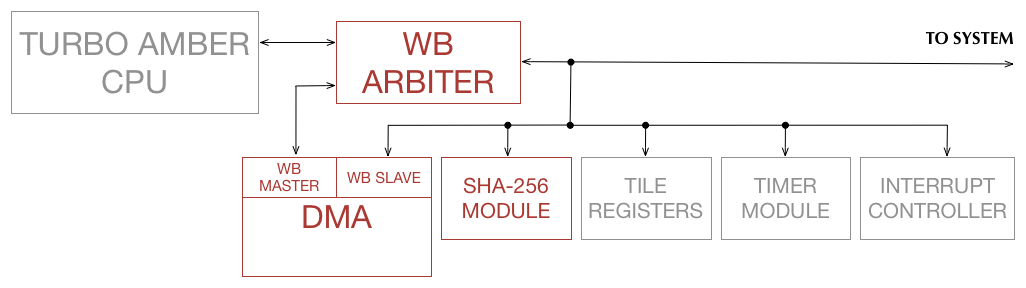
\includegraphics[width=1.0\textwidth]{Figures/Tile/HashingTile}
    \caption{SHMAC tile with SHA-256 accelerator and DMA. Added components are highlighted in red.}
    \label{fig:SHA-Tile}
\end{figure}

The new tile is derived from the Turbo Amber tile, which contains
a Turbo Amber CPU and peripherals such as an interrupt controller and timer modules, connected
together with a wishbone bus.

The SHA-256 accelerator and the DMA's slave interface and master interface is added to this bus.
With two masters connected to the Wishbone bus, arbitration is needed, thus an arbiter has been added as well.

\subsection{Wishbone Arbiter}
Since the DMA includes a wishbone master interface, a wishbone arbiter is also added to the tile.
The tile needs an arbiter to arbitrate between the DMA and the CPU on the wishbone bus.
For this purpose, the reference arbiter from the Wishbone Public Domain Library for VHDL % \cite{WBLibrary}
was adapted for use. This is a round-robin arbiter, illustrated in figure \ref{fig:WBArbiter}.

%
%For this project, the ARB0001a: 4 Level, Round-robin Arbiter from WISHBONE Public Domain Library for VHDL has been taken in use.
%Figure \cite{fig:WBArbiter} shows how the arbitration works, with Round-robin.
%The arbiter will in turn check each input master for bus requests, and grants access thereby.
%If a master has no request, the arbiter will continue to the next.
%For this project, only two masters are present.
%Arbitration normally take a full clock cycle.
%See \cite{WBLibrary} for detailed implementation.
%
\begin{figure}[htb]
    \centering
    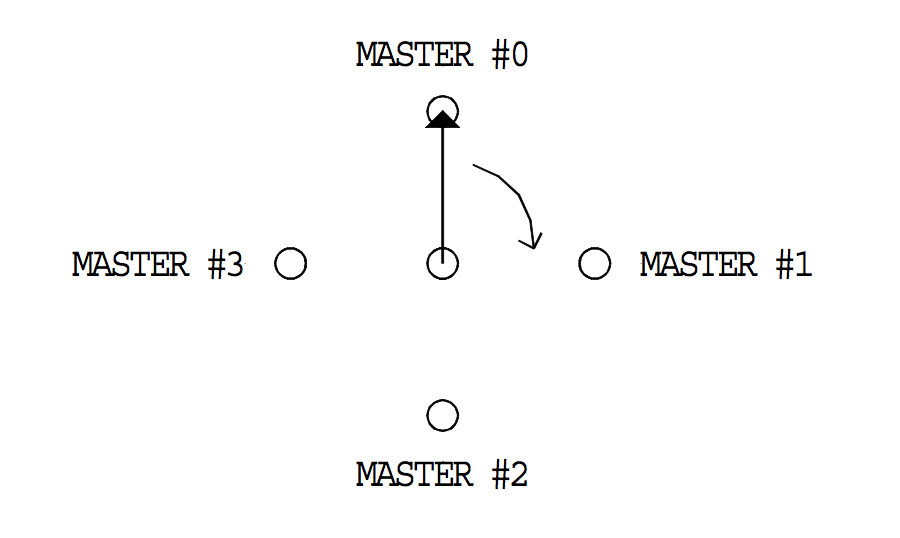
\includegraphics[width=1.0\textwidth]{Figures/Tile/WBArbiter}
    \caption{Wishbone Round-robin Arbiter, as seen in \cite{WBLibrary}.}
    \label{fig:WBArbiter}
\end{figure}

Round-robin arbiters work well in data acquisition systems where data is collected and placed into memory, since peripherals must often store data to memory.
The choice of this arbiter is because using an already established wishbone arbiter saves time for this project as opposed to desiging a new one, which may end up less efficient if done poorly.
%These are usually disadvantagous in said systems, but does not have the arbitration overhead \cite{WBLibrary}.\
%\todo{Discussion of alternatives. The following may be moved to future work.}

%An alternative to round-robin arbiters is priority arbiters.
%In the case of arbitration between a CPU and a DMA module, a priority arbiter may be used to achieve either burst mode, where the DMA gets full access on the bus until the transfer is finished, or transparent mode, where the CPU always has priority on the bus.
%The latter mode gives the slowest DMA transfer, but has been shown to give best overall system performance. \todo{Find those book sources again, if time. Current source does not validate claim of overall performance} \cite{DMA-lecture}.
%\todo{See NOTE answer in code}
% %**NOTE: Do we need this? Perhaps more on round-robin arbiters instead if more is needed.
% Torbjørn: Yes! I have been told all my time on academia that alternatives should be discussed and reasoned. Besides, didn't you just say so for what I wrote for the DMA Module under future work, that alternatives belongs home to Architecture chapter?! 

\subsection{SHA-256 Hashing Module}

The hashing module made for this project is a simple implementation of the algorithm described in
appendix \ref{app:hashing-algo}. It uses 65 cycles to compute the hash of its input data, running
one iteration of the SHA-256 compression function every cycle except cycle 65, which is used to
form new intermediate hash values from the results of the compression function.

In order for the module to remain generic, so that it can also be used in cryptography, it
is also not optimized specifically for bitcoin mining; specifically, this means that the module
does not support doing the two-pass hashing required by the bitcoin protocol, instead relying
on software to set up correct input data for the second pass. It also relies on software to
do the neccessary padding of the input data as required by the SHA-256 algorithm.

Even for generic SHA-256 hashing, several optimizations are possible. The SHA-256 algorithm
includes 64 32-bit constants, one for each round of the compression function. These can be
stored in a block RAM memory to save some logic resources \cite{optimizing-sha2}. However, this occupies valuable
block ram resources that, in SHMAC, is used both by CPUs and scratchpad memory tiles. Thus,
using block RAMs for optimization would place limits on how many tiles can be included in
a SHMAC design; indeed, it was observed when synthesizing large designs with many cores
that the FPGA would run out of block RAM before any other resources according to the synthesis logs.

Another optimization, that has already been mentioned in section \ref{sec:fpga-mining}, is
pipelining. This can increase the throughput to as much as one hash per cycle, but will require
a large amount of additional logic because of the amount of data required by each iteration
of the SHA-256 compression function. The state required would include 2048~bits of storage
for the expanded message block in addition to the two sets of 8 32~bit words needed for
state and the intermediate hash value respectively.

The module is controlled by the processor using a memory-mapped interface. This allows the use
of a DMA to offload data transfer between memory and the hashing module. The memory-mapped interface
provides registers for 512 bits of input and 256 bits of output data, in addition to control and
status registers. This interface can also be used for accelerators of other cryptographic hash
functions which processes input data of the same length and returns a hash of 256 bits or less,
such as RIPEMD-160 or RIPEMD-256 \cite{ripemd} or the still popular MD5 algorithm \cite{md5}.

With some work, the interface could be made even more generic in order to support algorithms
with other input and output sizes; a possibility would be to eliminate the input and output
registers completely in favour of using a DMA built into the module to move data of arbitrary
sizes into and out of the module.

Another, alternative interface to the module that was considered was using the co-processor interface
of the CPU to communicate with the module. The ARM instruction set supports up to 16 coprocessors,
which can be communicated with using the \texttt{mrc} and \texttt{mcr} instructions. Using this
interface for the hashing module would, however, have made it impossible to use a DMA to transfer
data to and from the module, making the hashing process much more dependent on the CPU, limiting
its benefits as an accelerator for offloading work from the processor.

% Figure

\subsection{DMA Module}

The DMA module was designed to test if separate data transfers with a DMA module could improve throughput and energy efficiency in the hashing process, freeing up the on-tile CPU for other work.

\begin{figure}[htb]
    \centering
    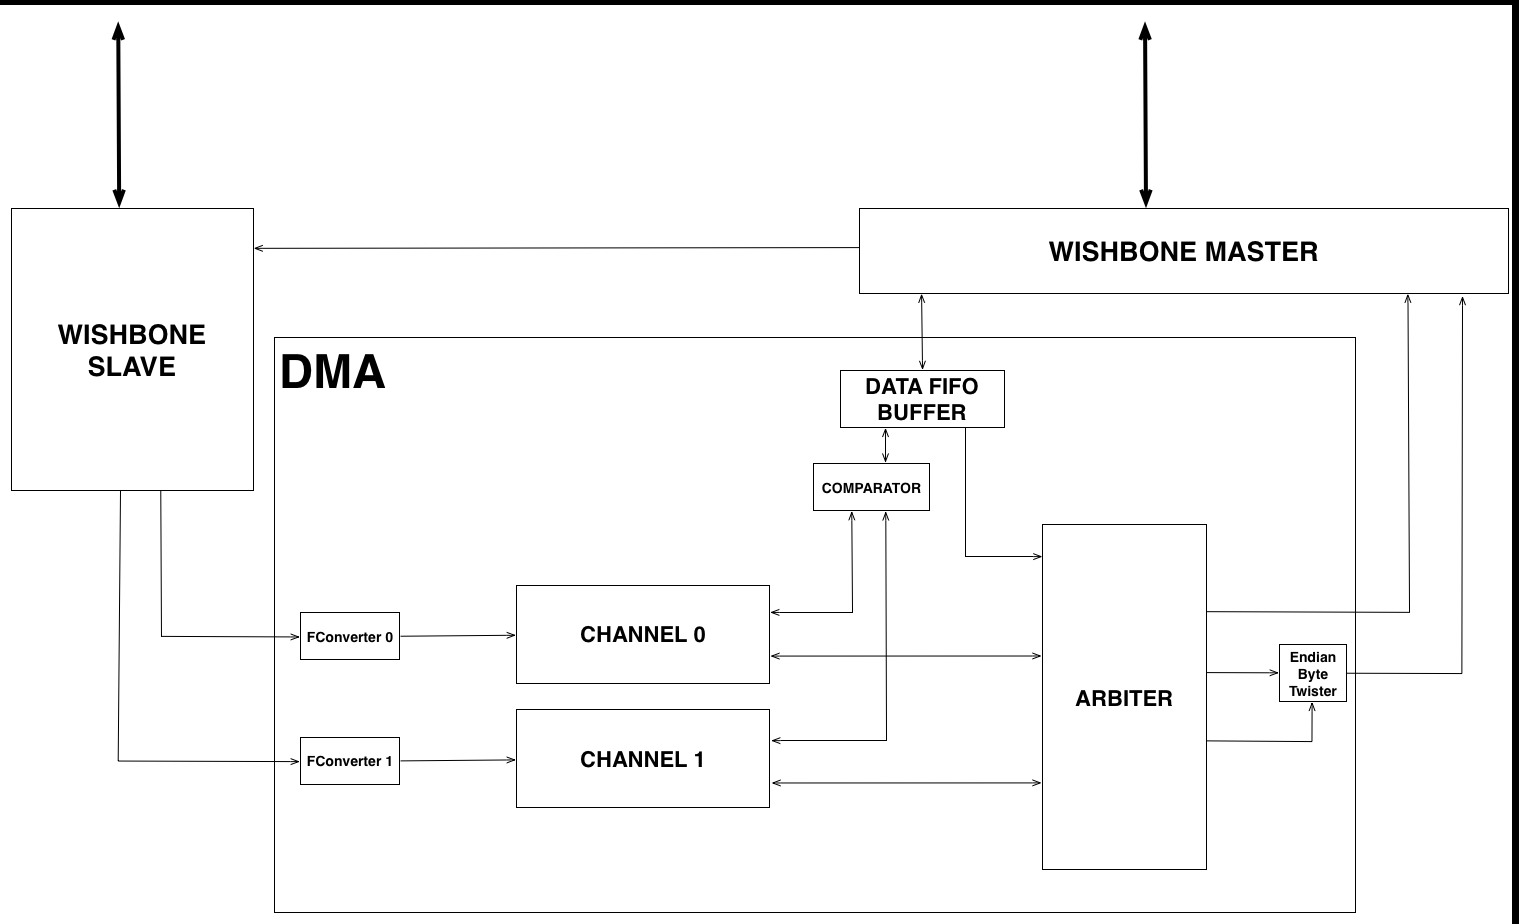
\includegraphics[width=1.0\textwidth]{Figures/DMA/DMATopview}
    \caption{DMA Topview, including Wishbone interface.}
    \label{fig:DMATop}
\end{figure}

The DMA module consists of the DMA logic, in addition to a wishbone slave interface for configuration
and a wishbone master interface for transferring data.

The DMA transfers words of 32-bit data using single wishbone transfers.  In addition, the DMA supports
swapping the endianness of the data it copies. This improves performance when used with the SHA256
accelerator, because the results from the accelerator are in big-endian
and must be converted to little-endian to give the correct results when used by the software running on the processor.
Converting endianness in software adds several additional instructions per hash, which are now avoided.

The Wishbone Slave consists of three registers for each DMA Channel, used for base source, base destination and detailing the transfer request.
When request is activated, the selected channel receives data from the slave, and executes the transfer.
An arbiter arbitrates between the channels if both are active.
Every single command, either load or store, are passed from the channels to the Wishbone master, where they are executed.
Loaded data is passed on to the corresponding channel, and a channel informs the WB master when it's finished, so that the slave interface is informed when final transfer is done executing.
The corresponding request detail register is modified, and the CPU is interrupted.

If endian swapping is active, the data bytes are simply swapped combinatorcially in a switch module before it is passed on to the wishbone master.

The current DMA Module only supports transfers of single 32-bit words, while the interconnect used in SHMAC supports 128-bit words.
This means four transfers are done on the network where ideally only one is would be needed. 
The reason to not expand to 128-bit blocks per individual transfer was due to the concern of forced alignment within the blocks.
While transferring aligned blocks of data from one memory location to another is common, switching a 32-bit word's position inside a block would not be possible for the DMA, if we were to expand the size without making considerable change to the DMA. 
We were concerned that this could prevent us from transferring data between neighbour registers on the tile.
Furthermore, it was concidered outside the scope of the project to further enhance the DMA Module, as the main idea was that this would enhance SHMAC generally, but not the hashing module.
In order to focus remaining project time on the Hashing module, and to have the ability to write to any register inside the tile, 32-bit data transfer were chosen.

\section{System architecture}
\label{sec:SHMAC_sys_arch}

SHA-256 hashing is sequential, with all data depending on each \todo{Was tired when writing. Fix tomorrow}round of calculation.
Aside from \todo{Is this described earlier yet?}optimizations, the only way to improve performance is running the hashing parallell on multiple independent tiles.

\subsection{5x4 architecture}
To test the accelerator, and how well it would run in such an environment, a 20~tile setup was used on SHMAC. It was decided to include the following tiles in the design:

\begin{itemize}
    \item 16 CPU tiles with on-tile DMA and SHA256 accelerator
    \item 2 scratchpad tiles
    \item 1 DRAM tile
    \item 1 I/O tile
\end{itemize}

The layout is illustrated in figure \ref{fig:5x4}. The I/O tile is placed to the
left of the first processor in the system, as only the first processor tile is used
for communicating with the host system. This gives the first processor a ``dedicated''
connection to the I/O tile, preventing data that is sent to the host from interferring
with data transfers needed for the hashing benchmark.

\begin{figure}[htb]
    \centering
    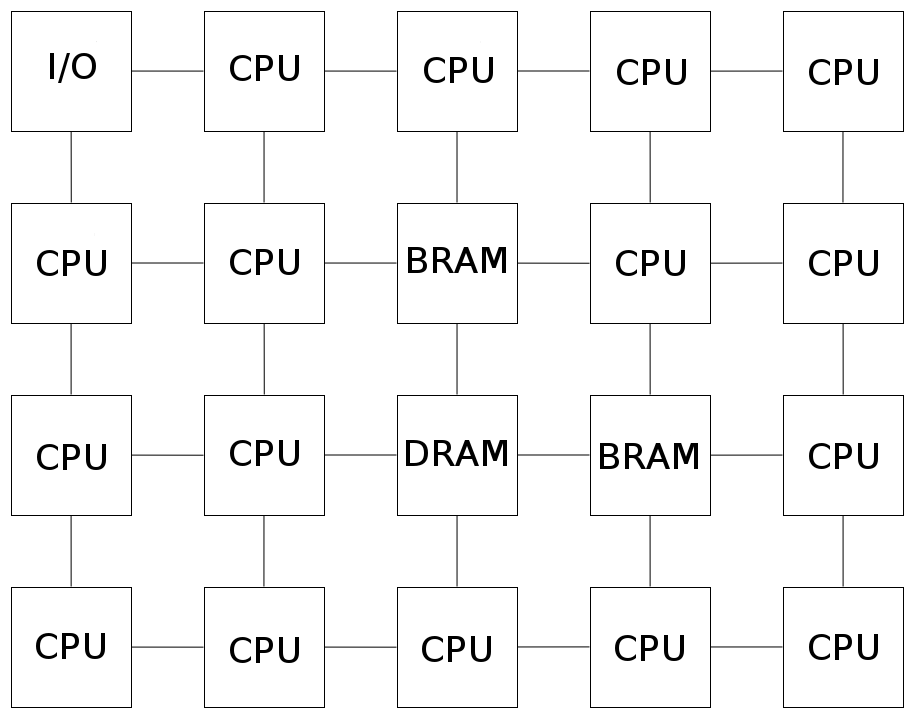
\includegraphics[width=0.5\textwidth]{Figures/Measurements/5x4}
    \caption{Test setup, using BRAM tiles as scratchpad and DRAM as main memory.}
    \label{fig:5x4}
\end{figure}

\subsection{15x2 architecture}
As testing uncovered a hardware bug in the implementation of the scratchpad tiles,
discussed in section \ref{sec:init-hw-results}, a second design had to be created
in order to measure the scaling of the performance when using accelerators.

The second design places all processor tiles in a single row. This causes all traffic
to the memory tiles, placed on the row below, to come from above, which bypasses the
scratchpad bug previously mentioned.

The design contains 14 CPU tiles and is illustrated in figure \ref{fig:15x2}. The
current implementation of SHMAC didn't allow more than 15 tiles on each row due
to only using 4 bits to represent each grid coordinate.\todo{Check sources}

\begin{figure}[htb]
    \centering
    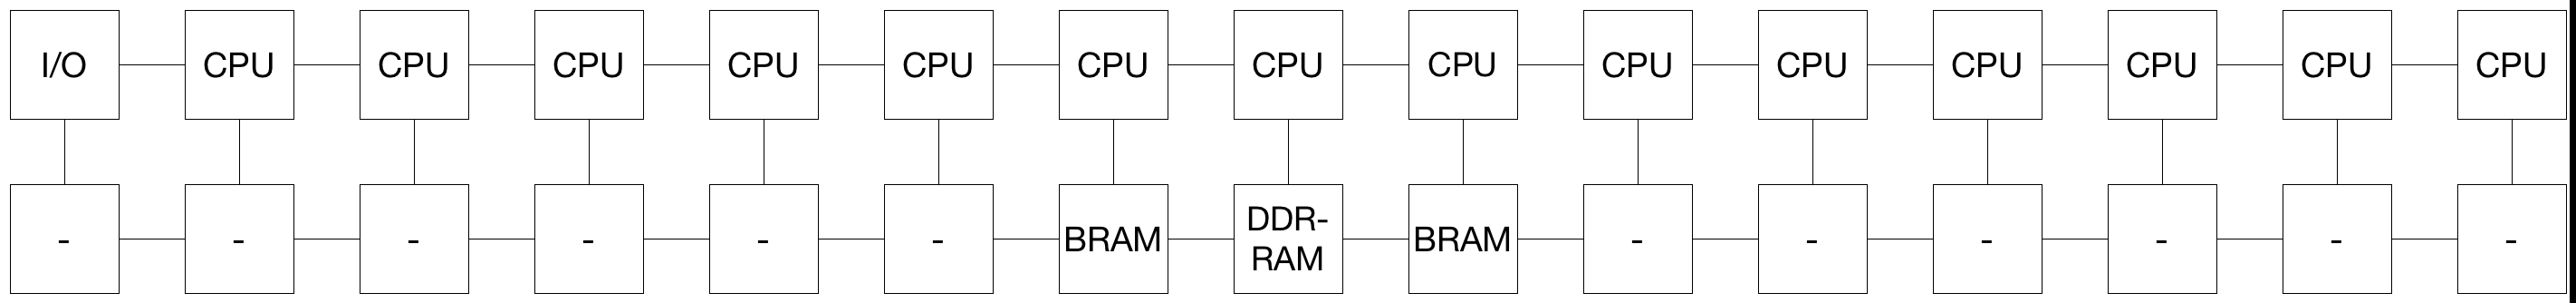
\includegraphics[width=1.0\textwidth]{Figures/Measurements/15x2}
    \caption{Alternative test setup.}
    \label{fig:15x2}
\end{figure}

The test designs were synthesized using Xilinx' Vivado software suite, version 2013.4, and
uploaded to a Versatile Express machine.


